\documentclass{standalone}
\usepackage{tikz}
\usetikzlibrary{patterns, positioning}


\begin{document}
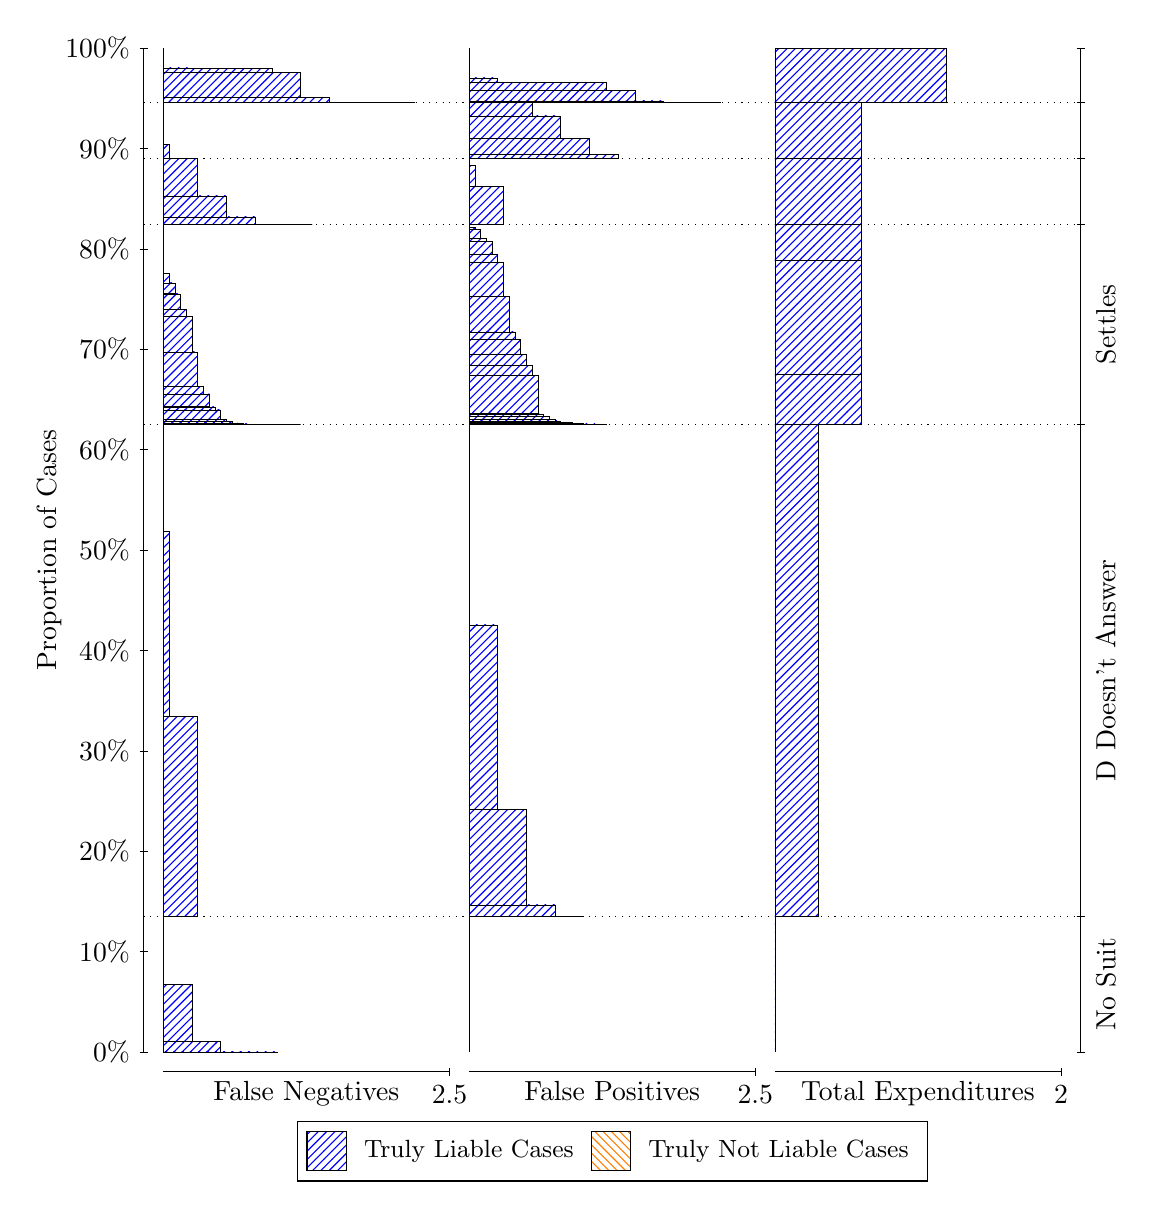
\begin{tikzpicture}
\draw[black, very thin] (1.5,1.75) -- (1.5,14.5);
\node[rotate=90, text=black, anchor=center] at (0.3, 8.125) {Proportion of Cases};
\draw[black, very thin] (1.45,1.75) -- (1.55,1.75);
\node[text=black, anchor=east] at (1.45, 1.75) {0\%};
\draw[black, very thin] (1.45,3.025) -- (1.55,3.025);
\node[text=black, anchor=east] at (1.45, 3.025) {10\%};
\draw[black, very thin] (1.45,4.3) -- (1.55,4.3);
\node[text=black, anchor=east] at (1.45, 4.3) {20\%};
\draw[black, very thin] (1.45,5.575) -- (1.55,5.575);
\node[text=black, anchor=east] at (1.45, 5.575) {30\%};
\draw[black, very thin] (1.45,6.85) -- (1.55,6.85);
\node[text=black, anchor=east] at (1.45, 6.85) {40\%};
\draw[black, very thin] (1.45,8.125) -- (1.55,8.125);
\node[text=black, anchor=east] at (1.45, 8.125) {50\%};
\draw[black, very thin] (1.45,9.4) -- (1.55,9.4);
\node[text=black, anchor=east] at (1.45, 9.4) {60\%};
\draw[black, very thin] (1.45,10.675) -- (1.55,10.675);
\node[text=black, anchor=east] at (1.45, 10.675) {70\%};
\draw[black, very thin] (1.45,11.95) -- (1.55,11.95);
\node[text=black, anchor=east] at (1.45, 11.95) {80\%};
\draw[black, very thin] (1.45,13.225) -- (1.55,13.225);
\node[text=black, anchor=east] at (1.45, 13.225) {90\%};
\draw[black, very thin] (1.45,14.5) -- (1.55,14.5);
\node[text=black, anchor=east] at (1.45, 14.5) {100\%};

\draw[black, very thin] (13.4,1.75) -- (13.4,14.5);
\draw[black, very thin] (13.35,1.75) -- (13.45,1.75);
\node[anchor=west] at (13.35, 1.75) {};
\draw[black, very thin] (13.35,3.4687) -- (13.45,3.4687);
\node[anchor=west] at (13.35, 3.4687) {};
\draw[black, very thin] (13.35,9.7225) -- (13.45,9.7225);
\node[anchor=west] at (13.35, 9.7225) {};
\draw[black, very thin] (13.35,12.261) -- (13.45,12.261);
\node[anchor=west] at (13.35, 12.261) {};
\draw[black, very thin] (13.35,13.1) -- (13.45,13.1);
\node[anchor=west] at (13.35, 13.1) {};
\draw[black, very thin] (13.35,13.81) -- (13.45,13.81);
\node[anchor=west] at (13.35, 13.81) {};
\draw[black, very thin] (13.35,14.5) -- (13.45,14.5);
\node[anchor=west] at (13.35, 14.5) {};

\draw[black, very thin, pattern color=blue, pattern=north east lines] (1.75,1.75) rectangle (3.2033,1.75);
\draw[black, very thin, pattern color=blue, pattern=north east lines] (1.75,1.75) rectangle (2.84,1.7512);
\draw[black, very thin, pattern color=blue, pattern=north east lines] (1.75,1.7512) rectangle (2.4767,1.8875);
\draw[black, very thin, pattern color=blue, pattern=north east lines] (1.75,1.8875) rectangle (2.1133,2.6106);
\draw[black, very thin, pattern color=orange, pattern=north west lines] (1.75,2.6106) rectangle (1.75,2.6106);
\draw[black, very thin, pattern color=blue, pattern=north east lines] (1.75,2.6106) rectangle (1.75,3.4687);
\draw[black, very thin, pattern color=blue, pattern=north east lines] (1.75,3.4687) rectangle (2.186,6.0166);
\draw[black, very thin, pattern color=blue, pattern=north east lines] (1.75,6.0166) rectangle (1.8227,8.3624);
\draw[black, very thin, pattern color=orange, pattern=north west lines] (1.75,8.3624) rectangle (1.75,8.3624);
\draw[black, very thin, pattern color=blue, pattern=north east lines] (1.75,8.3624) rectangle (1.75,9.7225);
\draw[black, very thin, pattern color=blue, pattern=north east lines] (1.75,9.7225) rectangle (3.494,9.7225);
\draw[black, very thin, pattern color=blue, pattern=north east lines] (1.75,9.7225) rectangle (3.3487,9.7225);
\draw[black, very thin, pattern color=blue, pattern=north east lines] (1.75,9.7225) rectangle (3.2033,9.7225);
\draw[black, very thin, pattern color=blue, pattern=north east lines] (1.75,9.7225) rectangle (3.1307,9.7225);
\draw[black, very thin, pattern color=blue, pattern=north east lines] (1.75,9.7225) rectangle (3.058,9.7225);
\draw[black, very thin, pattern color=blue, pattern=north east lines] (1.75,9.7225) rectangle (3.058,9.7225);
\draw[black, very thin, pattern color=blue, pattern=north east lines] (1.75,9.7225) rectangle (2.9853,9.7225);
\draw[black, very thin, pattern color=blue, pattern=north east lines] (1.75,9.7225) rectangle (2.9127,9.7225);
\draw[black, very thin, pattern color=blue, pattern=north east lines] (1.75,9.7225) rectangle (2.84,9.7264);
\draw[black, very thin, pattern color=blue, pattern=north east lines] (1.75,9.7264) rectangle (2.7673,9.7332);
\draw[black, very thin, pattern color=blue, pattern=north east lines] (1.75,9.7332) rectangle (2.6947,9.7332);
\draw[black, very thin, pattern color=blue, pattern=north east lines] (1.75,9.7332) rectangle (2.6947,9.7383);
\draw[black, very thin, pattern color=blue, pattern=north east lines] (1.75,9.7383) rectangle (2.622,9.7383);
\draw[black, very thin, pattern color=blue, pattern=north east lines] (1.75,9.7383) rectangle (2.622,9.7586);
\draw[black, very thin, pattern color=blue, pattern=north east lines] (1.75,9.7586) rectangle (2.5493,9.7792);
\draw[black, very thin, pattern color=blue, pattern=north east lines] (1.75,9.7792) rectangle (2.4767,9.9053);
\draw[black, very thin, pattern color=blue, pattern=north east lines] (1.75,9.9053) rectangle (2.404,9.9053);
\draw[black, very thin, pattern color=blue, pattern=north east lines] (1.75,9.9053) rectangle (2.404,9.9436);
\draw[black, very thin, pattern color=blue, pattern=north east lines] (1.75,9.9436) rectangle (2.3313,9.9451);
\draw[black, very thin, pattern color=blue, pattern=north east lines] (1.75,9.9451) rectangle (2.3313,10.108);
\draw[black, very thin, pattern color=blue, pattern=north east lines] (1.75,10.108) rectangle (2.3313,10.108);
\draw[black, very thin, pattern color=blue, pattern=north east lines] (1.75,10.108) rectangle (2.2587,10.108);
\draw[black, very thin, pattern color=blue, pattern=north east lines] (1.75,10.108) rectangle (2.2587,10.202);
\draw[black, very thin, pattern color=blue, pattern=north east lines] (1.75,10.202) rectangle (2.186,10.64);
\draw[black, very thin, pattern color=blue, pattern=north east lines] (1.75,10.64) rectangle (2.1133,11.087);
\draw[black, very thin, pattern color=blue, pattern=north east lines] (1.75,11.087) rectangle (2.0407,11.098);
\draw[black, very thin, pattern color=blue, pattern=north east lines] (1.75,11.098) rectangle (2.0407,11.179);
\draw[black, very thin, pattern color=blue, pattern=north east lines] (1.75,11.179) rectangle (1.968,11.185);
\draw[black, very thin, pattern color=blue, pattern=north east lines] (1.75,11.185) rectangle (1.968,11.378);
\draw[black, very thin, pattern color=blue, pattern=north east lines] (1.75,11.378) rectangle (1.968,11.378);
\draw[black, very thin, pattern color=blue, pattern=north east lines] (1.75,11.378) rectangle (1.8953,11.388);
\draw[black, very thin, pattern color=blue, pattern=north east lines] (1.75,11.388) rectangle (1.8953,11.517);
\draw[black, very thin, pattern color=blue, pattern=north east lines] (1.75,11.517) rectangle (1.8227,11.637);
\draw[black, very thin, pattern color=orange, pattern=north west lines] (1.75,11.637) rectangle (1.75,11.637);
\draw[black, very thin, pattern color=blue, pattern=north east lines] (1.75,11.637) rectangle (1.75,12.261);
\draw[black, very thin, pattern color=blue, pattern=north east lines] (1.75,12.261) rectangle (3.6393,12.261);
\draw[black, very thin, pattern color=blue, pattern=north east lines] (1.75,12.261) rectangle (3.276,12.261);
\draw[black, very thin, pattern color=blue, pattern=north east lines] (1.75,12.261) rectangle (2.9127,12.355);
\draw[black, very thin, pattern color=blue, pattern=north east lines] (1.75,12.355) rectangle (2.5493,12.623);
\draw[black, very thin, pattern color=blue, pattern=north east lines] (1.75,12.623) rectangle (2.186,13.1);
\draw[black, very thin, pattern color=orange, pattern=north west lines] (1.75,13.1) rectangle (1.75,13.1);
\draw[black, very thin, pattern color=blue, pattern=north east lines] (1.75,13.1) rectangle (2.186,13.102);
\draw[black, very thin, pattern color=blue, pattern=north east lines] (1.75,13.102) rectangle (1.8227,13.274);
\draw[black, very thin, pattern color=orange, pattern=north west lines] (1.75,13.274) rectangle (1.75,13.274);
\draw[black, very thin, pattern color=blue, pattern=north east lines] (1.75,13.274) rectangle (1.75,13.81);
\draw[black, very thin, pattern color=blue, pattern=north east lines] (1.75,13.81) rectangle (4.9473,13.81);
\draw[black, very thin, pattern color=blue, pattern=north east lines] (1.75,13.81) rectangle (4.584,13.81);
\draw[black, very thin, pattern color=blue, pattern=north east lines] (1.75,13.81) rectangle (4.2207,13.812);
\draw[black, very thin, pattern color=blue, pattern=north east lines] (1.75,13.812) rectangle (3.8573,13.875);
\draw[black, very thin, pattern color=blue, pattern=north east lines] (1.75,13.875) rectangle (3.494,14.189);
\draw[black, very thin, pattern color=blue, pattern=north east lines] (1.75,14.189) rectangle (3.1307,14.243);
\draw[black, very thin, pattern color=blue, pattern=north east lines] (1.75,14.243) rectangle (2.84,14.243);
\draw[black, very thin, pattern color=blue, pattern=north east lines] (1.75,14.243) rectangle (2.7673,14.244);
\draw[black, very thin, pattern color=blue, pattern=north east lines] (1.75,14.244) rectangle (2.4767,14.244);
\draw[black, very thin, pattern color=blue, pattern=north east lines] (1.75,14.244) rectangle (2.1133,14.248);
\draw[black, very thin, pattern color=orange, pattern=north west lines] (1.75,14.248) rectangle (1.75,14.248);
\draw[black, very thin, pattern color=blue, pattern=north east lines] (1.75,14.248) rectangle (1.75,14.5);
\draw[black, very thin, pattern color=orange, pattern=north west lines] (5.6333,1.75) rectangle (5.6333,1.75);
\draw[black, very thin, pattern color=blue, pattern=north east lines] (5.6333,1.75) rectangle (5.6333,3.4687);
\draw[black, very thin, pattern color=orange, pattern=north west lines] (5.6333,3.4687) rectangle (7.0867,3.4687);
\draw[black, very thin, pattern color=blue, pattern=north east lines] (5.6333,3.4687) rectangle (7.0867,3.4701);
\draw[black, very thin, pattern color=blue, pattern=north east lines] (5.6333,3.4701) rectangle (6.7233,3.6173);
\draw[black, very thin, pattern color=blue, pattern=north east lines] (5.6333,3.6173) rectangle (6.36,4.8288);
\draw[black, very thin, pattern color=blue, pattern=north east lines] (5.6333,4.8288) rectangle (5.9967,7.1746);
\draw[black, very thin, pattern color=blue, pattern=north east lines] (5.6333,7.1746) rectangle (5.6333,9.7225);
\draw[black, very thin, pattern color=orange, pattern=north west lines] (5.6333,9.7225) rectangle (7.3773,9.7225);
\draw[black, very thin, pattern color=blue, pattern=north east lines] (5.6333,9.7225) rectangle (7.3773,9.7242);
\draw[black, very thin, pattern color=orange, pattern=north west lines] (5.6333,9.7242) rectangle (7.232,9.7242);
\draw[black, very thin, pattern color=blue, pattern=north east lines] (5.6333,9.7242) rectangle (7.232,9.7259);
\draw[black, very thin, pattern color=orange, pattern=north west lines] (5.6333,9.7259) rectangle (7.0867,9.7259);
\draw[black, very thin, pattern color=blue, pattern=north east lines] (5.6333,9.7259) rectangle (7.0867,9.7292);
\draw[black, very thin, pattern color=blue, pattern=north east lines] (5.6333,9.7292) rectangle (7.014,9.7341);
\draw[black, very thin, pattern color=orange, pattern=north west lines] (5.6333,9.7341) rectangle (6.9413,9.7341);
\draw[black, very thin, pattern color=blue, pattern=north east lines] (5.6333,9.7341) rectangle (6.9413,9.7424);
\draw[black, very thin, pattern color=blue, pattern=north east lines] (5.6333,9.7424) rectangle (6.8687,9.7473);
\draw[black, very thin, pattern color=orange, pattern=north west lines] (5.6333,9.7473) rectangle (6.796,9.7473);
\draw[black, very thin, pattern color=blue, pattern=north east lines] (5.6333,9.7473) rectangle (6.796,9.7638);
\draw[black, very thin, pattern color=blue, pattern=north east lines] (5.6333,9.7638) rectangle (6.7233,9.7805);
\draw[black, very thin, pattern color=orange, pattern=north west lines] (5.6333,9.7805) rectangle (6.6507,9.7805);
\draw[black, very thin, pattern color=blue, pattern=north east lines] (5.6333,9.7805) rectangle (6.6507,9.8176);
\draw[black, very thin, pattern color=blue, pattern=north east lines] (5.6333,9.8176) rectangle (6.578,9.8549);
\draw[black, very thin, pattern color=blue, pattern=north east lines] (5.6333,9.8549) rectangle (6.5053,9.8562);
\draw[black, very thin, pattern color=orange, pattern=north west lines] (5.6333,9.8562) rectangle (6.5053,9.8562);
\draw[black, very thin, pattern color=blue, pattern=north east lines] (5.6333,9.8562) rectangle (6.5053,10.346);
\draw[black, very thin, pattern color=blue, pattern=north east lines] (5.6333,10.346) rectangle (6.4327,10.467);
\draw[black, very thin, pattern color=orange, pattern=north west lines] (5.6333,10.467) rectangle (6.36,10.467);
\draw[black, very thin, pattern color=blue, pattern=north east lines] (5.6333,10.467) rectangle (6.36,10.605);
\draw[black, very thin, pattern color=blue, pattern=north east lines] (5.6333,10.605) rectangle (6.2873,10.804);
\draw[black, very thin, pattern color=orange, pattern=north west lines] (5.6333,10.804) rectangle (6.2147,10.804);
\draw[black, very thin, pattern color=blue, pattern=north east lines] (5.6333,10.804) rectangle (6.2147,10.885);
\draw[black, very thin, pattern color=blue, pattern=north east lines] (5.6333,10.885) rectangle (6.2147,10.896);
\draw[black, very thin, pattern color=blue, pattern=north east lines] (5.6333,10.896) rectangle (6.142,10.896);
\draw[black, very thin, pattern color=blue, pattern=north east lines] (5.6333,10.896) rectangle (6.142,11.344);
\draw[black, very thin, pattern color=blue, pattern=north east lines] (5.6333,11.344) rectangle (6.0693,11.781);
\draw[black, very thin, pattern color=blue, pattern=north east lines] (5.6333,11.781) rectangle (5.9967,11.875);
\draw[black, very thin, pattern color=blue, pattern=north east lines] (5.6333,11.875) rectangle (5.924,12.04);
\draw[black, very thin, pattern color=blue, pattern=north east lines] (5.6333,12.04) rectangle (5.8513,12.078);
\draw[black, very thin, pattern color=blue, pattern=north east lines] (5.6333,12.078) rectangle (5.8513,12.078);
\draw[black, very thin, pattern color=blue, pattern=north east lines] (5.6333,12.078) rectangle (5.7787,12.078);
\draw[black, very thin, pattern color=blue, pattern=north east lines] (5.6333,12.078) rectangle (5.7787,12.204);
\draw[black, very thin, pattern color=blue, pattern=north east lines] (5.6333,12.204) rectangle (5.706,12.225);
\draw[black, very thin, pattern color=blue, pattern=north east lines] (5.6333,12.225) rectangle (5.6333,12.261);
\draw[black, very thin, pattern color=orange, pattern=north west lines] (5.6333,12.261) rectangle (6.0693,12.261);
\draw[black, very thin, pattern color=blue, pattern=north east lines] (5.6333,12.261) rectangle (6.0693,12.738);
\draw[black, very thin, pattern color=blue, pattern=north east lines] (5.6333,12.738) rectangle (5.706,13.005);
\draw[black, very thin, pattern color=blue, pattern=north east lines] (5.6333,13.005) rectangle (5.6333,13.1);
\draw[black, very thin, pattern color=orange, pattern=north west lines] (5.6333,13.1) rectangle (7.5227,13.1);
\draw[black, very thin, pattern color=blue, pattern=north east lines] (5.6333,13.1) rectangle (7.5227,13.147);
\draw[black, very thin, pattern color=blue, pattern=north east lines] (5.6333,13.147) rectangle (7.1593,13.357);
\draw[black, very thin, pattern color=blue, pattern=north east lines] (5.6333,13.357) rectangle (6.796,13.637);
\draw[black, very thin, pattern color=blue, pattern=north east lines] (5.6333,13.637) rectangle (6.4327,13.808);
\draw[black, very thin, pattern color=blue, pattern=north east lines] (5.6333,13.808) rectangle (6.0693,13.81);
\draw[black, very thin, pattern color=orange, pattern=north west lines] (5.6333,13.81) rectangle (8.8307,13.81);
\draw[black, very thin, pattern color=blue, pattern=north east lines] (5.6333,13.81) rectangle (8.8307,13.81);
\draw[black, very thin, pattern color=blue, pattern=north east lines] (5.6333,13.81) rectangle (8.4673,13.811);
\draw[black, very thin, pattern color=orange, pattern=north west lines] (5.6333,13.811) rectangle (8.4673,13.811);
\draw[black, very thin, pattern color=blue, pattern=north east lines] (5.6333,13.811) rectangle (8.4673,13.811);
\draw[black, very thin, pattern color=blue, pattern=north east lines] (5.6333,13.811) rectangle (8.104,13.812);
\draw[black, very thin, pattern color=orange, pattern=north west lines] (5.6333,13.812) rectangle (8.104,13.812);
\draw[black, very thin, pattern color=blue, pattern=north east lines] (5.6333,13.812) rectangle (8.104,13.829);
\draw[black, very thin, pattern color=blue, pattern=north east lines] (5.6333,13.829) rectangle (7.7407,13.829);
\draw[black, very thin, pattern color=orange, pattern=north west lines] (5.6333,13.829) rectangle (7.7407,13.829);
\draw[black, very thin, pattern color=blue, pattern=north east lines] (5.6333,13.829) rectangle (7.7407,13.965);
\draw[black, very thin, pattern color=blue, pattern=north east lines] (5.6333,13.965) rectangle (7.3773,13.965);
\draw[black, very thin, pattern color=blue, pattern=north east lines] (5.6333,13.965) rectangle (7.3773,14.062);
\draw[black, very thin, pattern color=blue, pattern=north east lines] (5.6333,14.062) rectangle (7.014,14.067);
\draw[black, very thin, pattern color=blue, pattern=north east lines] (5.6333,14.067) rectangle (6.6507,14.067);
\draw[black, very thin, pattern color=orange, pattern=north west lines] (5.6333,14.067) rectangle (6.36,14.067);
\draw[black, very thin, pattern color=blue, pattern=north east lines] (5.6333,14.067) rectangle (6.36,14.067);
\draw[black, very thin, pattern color=blue, pattern=north east lines] (5.6333,14.067) rectangle (6.2873,14.067);
\draw[black, very thin, pattern color=orange, pattern=north west lines] (5.6333,14.067) rectangle (5.9967,14.067);
\draw[black, very thin, pattern color=blue, pattern=north east lines] (5.6333,14.067) rectangle (5.9967,14.122);
\draw[black, very thin, pattern color=orange, pattern=north west lines] (5.6333,14.122) rectangle (5.6333,14.122);
\draw[black, very thin, pattern color=blue, pattern=north east lines] (5.6333,14.122) rectangle (5.6333,14.5);
\draw[black, very thin, pattern color=orange, pattern=north west lines] (9.5167,1.75) rectangle (9.5167,1.75);
\draw[black, very thin, pattern color=blue, pattern=north east lines] (9.5167,1.75) rectangle (9.5167,3.4687);
\draw[black, very thin, pattern color=orange, pattern=north west lines] (9.5167,3.4687) rectangle (10.062,3.4687);
\draw[black, very thin, pattern color=blue, pattern=north east lines] (9.5167,3.4687) rectangle (10.062,9.7225);
\draw[black, very thin, pattern color=orange, pattern=north west lines] (9.5167,9.7225) rectangle (10.607,9.7225);
\draw[black, very thin, pattern color=blue, pattern=north east lines] (9.5167,9.7225) rectangle (10.607,10.354);
\draw[black, very thin, pattern color=orange, pattern=north west lines] (9.5167,10.354) rectangle (10.607,10.354);
\draw[black, very thin, pattern color=blue, pattern=north east lines] (9.5167,10.354) rectangle (10.607,11.801);
\draw[black, very thin, pattern color=orange, pattern=north west lines] (9.5167,11.801) rectangle (10.607,11.801);
\draw[black, very thin, pattern color=blue, pattern=north east lines] (9.5167,11.801) rectangle (10.607,12.261);
\draw[black, very thin, pattern color=orange, pattern=north west lines] (9.5167,12.261) rectangle (10.607,12.261);
\draw[black, very thin, pattern color=blue, pattern=north east lines] (9.5167,12.261) rectangle (10.607,13.1);
\draw[black, very thin, pattern color=orange, pattern=north west lines] (9.5167,13.1) rectangle (10.607,13.1);
\draw[black, very thin, pattern color=blue, pattern=north east lines] (9.5167,13.1) rectangle (10.607,13.81);
\draw[black, very thin, pattern color=orange, pattern=north west lines] (9.5167,13.81) rectangle (11.697,13.81);
\draw[black, very thin, pattern color=blue, pattern=north east lines] (9.5167,13.81) rectangle (11.697,13.812);
\draw[black, very thin, pattern color=orange, pattern=north west lines] (9.5167,13.812) rectangle (11.697,13.812);
\draw[black, very thin, pattern color=blue, pattern=north east lines] (9.5167,13.812) rectangle (11.697,14.5);
\draw[black, dotted] (1.5,3.4687) -- (13.4,3.4687);
\draw[black, dotted] (1.5,9.7225) -- (13.4,9.7225);
\draw[black, dotted] (1.5,12.261) -- (13.4,12.261);
\draw[black, dotted] (1.5,13.1) -- (13.4,13.1);
\draw[black, dotted] (1.5,13.81) -- (13.4,13.81);
\draw[black, very thin] (1.75,1.5) -- (5.3833,1.5);
\node[text=black, anchor=north] at (3.5667, 1.5) {False Negatives};
\draw[black, very thin] (5.3833,1.45) -- (5.3833,1.55);
\node[text=black, anchor=north] at (5.3833, 1.45) {2.5};

\draw[black, very thin] (5.6333,1.5) -- (9.2667,1.5);
\node[text=black, anchor=north] at (7.45, 1.5) {False Positives};
\draw[black, very thin] (9.2667,1.45) -- (9.2667,1.55);
\node[text=black, anchor=north] at (9.2667, 1.45) {2.5};

\draw[black, very thin] (9.5167,1.5) -- (13.15,1.5);
\node[text=black, anchor=north] at (11.333, 1.5) {Total Expenditures};
\draw[black, very thin] (13.15,1.45) -- (13.15,1.55);
\node[text=black, anchor=north] at (13.15, 1.45) {2};

\node[text=black, centered, rotate=90] at (13.72, 2.6094) {No Suit};
\node[text=black, centered, rotate=90] at (13.72, 6.5956) {D Doesn't Answer};
\node[text=black, centered, rotate=90] at (13.72, 10.992) {Settles};




\draw (7.449999999999999,1.5) node[draw=none] (baseCoordinate) {};
\begin{scope}[align=center]
        \matrix[scale=0.5, draw=black, below=0.5cm of baseCoordinate, nodes={draw}, column sep=0.1cm]{
            \node[rectangle, draw, minimum width=0.5cm, minimum height=0.5cm, pattern color=blue, pattern=north east lines] {}; &
            \node[draw=none, font=\small, text=black] (B) {Truly Liable Cases}; &
            \node[rectangle, draw, minimum width=0.5cm, minimum height=0.5cm, pattern color=orange, pattern=north west lines] {}; &
            \node[draw=none, font=\small, text=black] (B) {Truly Not Liable Cases}; \\
            };
\end{scope}

\end{tikzpicture}
\end{document}